\documentclass[tp]{lcc}

% add latex preamble
% para la bibliografía se requiere biber y configurar texstudio

% Latex packages
\usepackage[utf8]{inputenc}
\usepackage[T1]{fontenc} % para copiar acentos en español del pdf y permite acentos en las notas
\usepackage[spanish]{babel}
\usepackage[per-mode = symbol]{siunitx} % para manejar las unidades
\usepackage{multimedia} % to add videos with \movie command
\usepackage{multirow}
\usepackage{graphicx}
\usepackage{xcolor}
\usepackage{amsmath} % bmatrix
\usepackage[makeroom]{cancel} % \cancel to cancel terms in math equations
\renewcommand{\CancelColor}{\color{red}} % set red color for \cancel command
\usepackage[caption=false]{subfig} % caption = false elimina la palabra "Figura" del caption
\usepackage{import} % para el comando import (se usa para pdf_tex)
\captionsetup[subfigure]{labelformat=empty} % remover el indice del caption de la subfigura
\usepackage{booktabs} % \toprule \midrule \bottomrule
\usepackage[backend=biber]{biblatex} % set biber to format references. Must configure Biber in Texstudio
\usepackage{csquotes} % to remove warning triggered by biblatex and babel
\usepackage{algorithm} % to put captions to the algorithmics environmets
\usepackage{algpseudocode} % to write algorithm
\usepackage{tikz} % to use tikz
\usetikzlibrary{fit} % to fit a node around other nodes in tikz
\usepackage[export]{adjustbox} % valign in subfloat
\usepackage{colortbl} % to paint cells in a table

% Color commands for annotations
\newcommand\TODO[1]{\textbf{\textcolor{red}{#1}}} %  TODO notes

% Graphic paths
\graphicspath{{./images/}}

% listings configuration for C code
\usepackage{listings} % code
\definecolor{commentgreen}{RGB}{2,112,10}
\definecolor{eminence}{RGB}{108,48,130}
\definecolor{weborange}{RGB}{255,165,0}
\definecolor{frenchplum}{RGB}{129,20,83}

\lstset{ % spanish characters for listings package
	inputencoding=latin1,
    columns=fullflexible,
	breaklines=true,
	tabsize=2,
	showstringspaces=false,
	basicstyle=\ttfamily,
	backgroundcolor=\color{lightgray}, % Choose background color
	literate={á}{{\'a}}1
	{ã}{{\~a}}1
	{é}{{\'e}}1
	{ó}{{\'o}}1
	{í}{{\'i}}1
	{ñ}{{\~n}}1
	{¡}{{!`}}1
	{¿}{{?`}}1
	{ú}{{\'u}}1
	{Í}{{\'I}}1
	{Ó}{{\'O}}1
    {-}{-}1
}

\lstdefinestyle{cpp}{ % spanish characters for listings package
    language=C++,
   	commentstyle=\color{commentgreen},
    keywordstyle=\color{eminence},
    stringstyle=\color{red},
    emph={int,char,double,float,unsigned,void,bool},
    emphstyle={\color{blue}}
}

\lstdefinestyle{bash}{ % spanish characters for listings package
	language=Bash
}

\lstdefinestyle{xml}{
	language=XML,
	morekeywords={encoding,xs:schema,xs:element,xs:complexType,xs:sequence,xs:attribute}
}

\lstdefinestyle{cmake}{
	language=make, % there is no cmake support in listings
}

\lstdefinestyle{python}{
    language=python,
}


%%%%% PARA QUE EN LAS TABLAS SE PUEDA PONER UN SALTO DE LINEA DENTRO DE UNA CELDA
\newcommand{\specialcell}[2][c]{%
    \begin{tiny}
        \begin{tabular}[#1]{@{}c@{}}#2\end{tabular}  
    \end{tiny}
}
%%%%%%%%%%%%%%%%%%%%%%%%%%%%%%%%%%%%%%%%%%%%%%%%%%%%%%%%%%%%%%%%%%%%%%%%

%%%%% PARA QUE LAS TABLAS TENGAN TODAS LAS COLUMNAS CENTRADAS Y DE IGUAL TAMAÑO
\usepackage{tabularx}
\renewcommand{\tabularxcolumn}[1]{>{\centering\arraybackslash}m{#1}}
%%%%%%%%%%%%%%%%%%%%%%%%%%%%%%%%%%%%%%%%%%%%%%%%%%%%%%%%%%%%%%%%%%%%%%%%



% add math preamble
\usepackage{amsmath}
\usepackage{amssymb}
\usepackage{amsopn}
\usepackage{mathtools}

% math
\renewcommand{\vec}[1]{\boldsymbol{\mathbf{#1}}}
\newcommand{\norm}[1]{\lVert#1\rVert}

% Declare arg max and arg min functionss
\DeclareMathOperator*{\argmax}{arg\,max}
\DeclareMathOperator*{\argmin}{arg\,min}

% Homogeneous decoration function
\newcommand{\homo}[1]{\dot{#1}}


% Declare projection as math function
\DeclareMathOperator{\proj}{proj}
\newcommand{\fromCoord}[2]{{#1}_\mathrm{#2}}
\newcommand{\toCoord}[2]{\prescript{\mathrm{#2}}{}{#1}}
\newcommand{\worldCoordSystem}{\mathrm{w}}
\newcommand{\bodyCoordSystem}{\mathrm{B}}
\newcommand{\cameraCoordSystem}{\mathrm{c}}
\newcommand{\point}{\vec{p}}
\newcommand{\worldPoint}{\toCoord{\point}{\worldCoordSystem}}
\newcommand{\imagePoint}{\vec{u}}
\newcommand{\cameraPoint}{\toCoord{\point}{\cameraCoordSystem}}
\newcommand{\homoWorldPoint}{\toCoord{\homo{\point}}{\worldCoordSystem}}
\newcommand{\homoImagePoint}{\homo{\imagePoint}}
\newcommand{\homoCameraPoint}{\toCoord{\homo{\point}}{\cameraCoordSystem}}
\newcommand{\measurement}{\vec{z}}
\newcommand{\prediction}{\hat{\vec{z}}}
\newcommand{\seMatrix}{\vec{\xi}}
\newcommand{\transform}[2]{\toCoord{\fromCoord{\seMatrix}{#2}}{#1}}
\newcommand{\pointCoord}[1]{\toCoord{\point}{#1}}
\newcommand{\rotation}{\vec{R}}
\newcommand{\rotationCoord}[2]{\toCoord{\fromCoord{\rotation}{#2}}{#1}}
\newcommand{\translation}{\vec{t}}
\newcommand{\translationCoord}[2]{\toCoord{\fromCoord{\translation}{#2}}{#1}}
\newcommand{\intrinsicMatrix}{\vec{K}}
\newcommand{\principalPoint}{\vec{c}}
\newcommand{\reprojectionError}{u}
\newcommand{\projectionMatrix}{\vec{P}}
\newcommand{\cameraCenter}{\vec{o}}
\newcommand{\essentialMatrix}{\vec{E}}
\newcommand{\inverse}[1]{{#1}^{-1}}

% Motion model
\newcommand{\position}{\vec{p}}
\newcommand{\orientationQuaternion}{\vec{q}}
\newcommand{\predictedPosition}{\hat{\vec{p}}}
\newcommand{\predictedOrientationQuaternion}{\hat{\vec{q}}}
\newcommand{\linearVelocity}{\vec{v}}
\newcommand{\angularVelocity}{\vec{\omega}}

\DeclareMathOperator{\slerpOp}{slerp}
\newcommand{\slerp}[1]{\slerpOp{\left( #1 \right)}}

% Map structure
\newcommand{\map}{M}
\newcommand{\keyframesSet}{K}
\newcommand{\mapPointsSet}{P}
\newcommand{\observedMapPoints}{O}
\newcommand{\covisibilityKeyframes}{CK}
\newcommand{\localMap}{local\_map}



% Bundle Adjutment
\newcommand{\update}{\vec{\delta}}
\newcommand{\incremental}{\hat{\update}}


% Loop Closure names

% scaled operators and letters to fancy view
\newcommand{\sminus}{\scalebox{0.5}[1.0]{$-$}}
\newcommand{\splus}{\scalebox{0.6}[0.6]{$+$}}
\newcommand{\curr}{c}
\newcommand{\sind}[1]{\scalebox{0.6}[0.6]{$#1$}}
\newcommand{\ind}[1]{\scalebox{0.7}[0.7]{$#1$}}

\newcommand{\keyframe}{\vec{K}}
\newcommand{\bowVector}{\vec{v}}
\newcommand{\lcError}{\vec{\Omega}}
\newcommand{\relativeTransformation}{\seMatrix}
\DeclareMathOperator{\interpolate}{interpolate}

\newcommand{\relativeMotion}{\vec{\delta}}
\newcommand{\groundTruth}[1]{{#1}^{*}}



% definición del operador rot()
\DeclareMathOperator{\rotationOp}{rot}
\newcommand{\getRotation}[1]{\rotationOp{\left( #1 \right)}}

\DeclareMathOperator{\translationOp}{trans}
\newcommand{\getTranslation}[1]{\translationOp{\left( #1 \right)}}









\codigo{R-521}
\materia{Robótica Móvil}
\titulo{EKF para Localización de un Robot Móvil}

\soluciones
\commentstrue


\usepackage{biblatex}
%\addbibresource{refs.bib}

\begin{document}
	\maketitle
	
	
	\section{Introducción}
	
	El objetivo del Trabajo Práctico es comprender cómo funciona EKF para la localización de un robot móvil y desarrollar una implementación funcional del mismo.
	
	Para esta tarea se utilizará un framework de Python provisto por la cátedra. Aunque se alienta a que se desarrolle en ROS2 y Gazebo. \footnote{Este trabajo práctico está basado en el trabajo práctico del curso CSE 571 - Robotics \url{https://courses.cs.washington.edu/courses/cse571/20sp/homeworks/HW2.pdf}.}
	
	Material de lectura útil: slides de las clases, Capítulos 3,4,5,7 \& 8 del libro Probabilistic Robotics, Thrun, Burgard and Fox.
	
	
	\section{Entrega}
	\begin{itemize}
		\item Se debe proveer un repositorio git que contenga el código desarrollado, una imagen docker y un archivo \lstinline{README.md} con las instrucciones de compilación y ejecución.
		
		\item Se debe entregar un informe en Lyx o \LaTeX\  explicando el trabajo realizado y analizando los resultados obtenidos.
	\end{itemize}

	
	\section{Ejercicios}
	
	
	Implementar un filtro de Kalman extendido (EKF) y filtro de partículas (PF) para localizar un robot basado en puntos de referencia. Usaremos el modelo de movimiento basado en la odometría que derivó en la pregunta 1.2. Suponemos que hay puntos de referencia presentes en el entorno del robot. El robot recibe los rumbos (ángulos) a los puntos de referencia y la ID de la puntos de referencia como observaciones: (rumbo, ID de punto de referencia).
	
	Asumimos un modelo de ruido para el modelo de movimiento de odometría con parámetros $\alpha$ (PR Tabla 5.6) y un modelo separado modelo de ruido para las observaciones de rumbo con parámetro $\beta$ (PR Sección 6.6). La observación de ID de punto de referencia es sin ruido. Consulte el código de inicio proporcionado para obtener detalles de implementación.
	
	En cada paso de tiempo, el robot comienza desde el estado actual y se mueve de acuerdo con la entrada de control. El robot luego recibe una observación histórica del mundo. Utilizará esta información para localizar el robot sobre el
	secuencia de tiempo completo con un EKF y PF.
	
	\begin{figure}[!htbp]
		\centering
		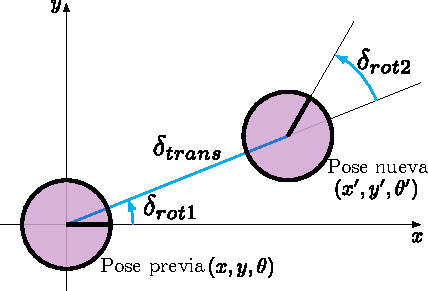
\includegraphics[width=0.5\textwidth]{./images/odometry_as_controls.pdf}
		\label{fig:odometry-base-motion-model}
	\end{figure}
	
	\ejercicio  Determinar de forma analítica el radio del camino circular que realiza el robot al ajustar la velocidad lineal y angular a valores constantes. Realizar el cálculo para dos velocidades cualquieras teniendo en cuenta las velocidades máximas del robot.
	
	\begin{nota}
		Los límites de velocidad y los parámetros cinemáticos (el radio de la rueda R y la distancia entre ruedas b) de los diferentes modelos del robot TurtleBot3 se obtienen de las especificaciones\footnote{\url{https://emanual.robotis.com/docs/en/platform/turtlebot3/features/}}.
	\end{nota}
	
	\ejercicio  Calcular la velocidad lineal y angular para que el robot realice un camino circular con un radio a elección entre \SI{0.5}{\meter} y \SI{1.5}{\meter}.
	
	\ejercicio  Calcular las velocidades lineales y angulares de las ruedas (izquierda y derecha) del robot para el camino circular del punto anterior.
	
	\ejercicio Generar un registro (log) de odometría y velocidad del robot, para lo cual hay que ejecutar nuevamente
	la simulación y utilizar el script ’dump odom.py’. Este script muestra en pantalla 6 columnas con los siguientes datos: tiempo (timestamp), coordenadas x, y, orientación, velocidad lineal y angular.
	
	\ejercicio Obtener un registro de datos con el robot en movimiento mediante teleoperación por teclado. Para guardar los datos generados por el script hay que redireccionar la salida a un archivo como:
	
	\begin{lstlisting}[style=bash] 
		./dump_odom.py > log.txt
	\end{lstlisting}
	
	\ejercicio Escribir un script en Python que cargue los datos del archivo log y genere gráficos de:
	\begin{enumerate}
		\item el camino seguido por el robot,
		\item la trayectoria (pose respecto al tiempo), y
		\item la velocidad del robot respecto al tiempo.
	\end{enumerate} 
	
	\begin{nota}
		Utilizar una relación de aspecto 1:1 para el gráfico del camino y evitar en lo posible el registro de datos iguales a cero.
	\end{nota}
	
	\ejercicio Obtener otro registro de datos para un camino circular del robot y graficar el camino y la trayectoria.
	
	\ejercicio Marcar tres puntos cualquiera en el gráfico del camino del robot y sus correspondientes puntos en la trayectoria. Elegir puntos diferentes al inicio y final del camino.
	
	
	En base a los gráficos anteriores:
	
	\begin{enumerate}
		
		\item ¿Cuáles son los rangos de valores de las coordenadas x e y y por qué?
		
		\item  ¿Cuál es el rango de valores de la orientación del robot y por qué?
		
		\item Obtener diferentes registros y gráficos para caminos circulares con diferentes valores (positivos y negativos) de velocidades lineales y angulares (utilizar todas las combinaciones de signos posibles). Indicar en los gráficos el sentido de avance del robot.
		
		\item Describir cuál sería la secuencia de comandos de velocidad a aplicar al robot para seguir uno de los caminos mostrados en la Figura~\ref{fig:trajectories} (elegir solo uno).
		
		\begin{nota}
			Para setear los comandos de velocidad por un tiempo determinado se puede utilizar el comando \lstinline[style=bash]{ros2 topic pub} con los argumentos \lstinline[style=bash]{-1} y \lstinline[style=bash]{--keep-alive}.
		\end{nota}
		
	\end{enumerate}
	

	\ejercicio El mundo deberá contar con varios cilindros de un mismo radio $r$. Los cilindros deben estar distribuidos en el entorno y ser todos observados por el láser del robot al momento de inicio de la simulación.
	
	Utilizar una medición láser para generar un mapa de la escena observada por el robot en simulación. Para esto deberá detectar los cilindros en la medición laser obtenida. Cada cilindro será utilizado como un landmark en el mapa virtual del robot. Deberá estimar el centro del cilindro, dicha posición será la posición de un landmark en el mapa virtual del robot. Debera crear un mapa de landmarks, publicarlo y visualizarlo en RVIZ utilizando el marker de cilindro.
	Obtenga una captura de pantalla de RViz donde se visualice las mediciones del láser y los landmarks reconstruidos.
	
	
	\printbibliography
	
\end{document}
